São elementos de fundação executados em concreto armado com altura reduzida em relação às dimensões da base e caracteriza-se, principalmente, por trabalhar à flexão.

Tipos de sapatas:

\begin{itemize}
	\item Sapata isolada;
	\item Sapata conjugada ou viga de fundação;
	\item Sapata corrida;
	\item Sapata com viga de equilíbrio ou sapata com viga alavanca;
	\item Sapata associada ou radier parcial.
\end{itemize}

\subsubsection{Sapata isolada}

São aquelas que atendem a um único pilar.

\begin{figure}[htb]
	\begin{center}
	\caption{Sapata isolada em perpspectiva.}
    	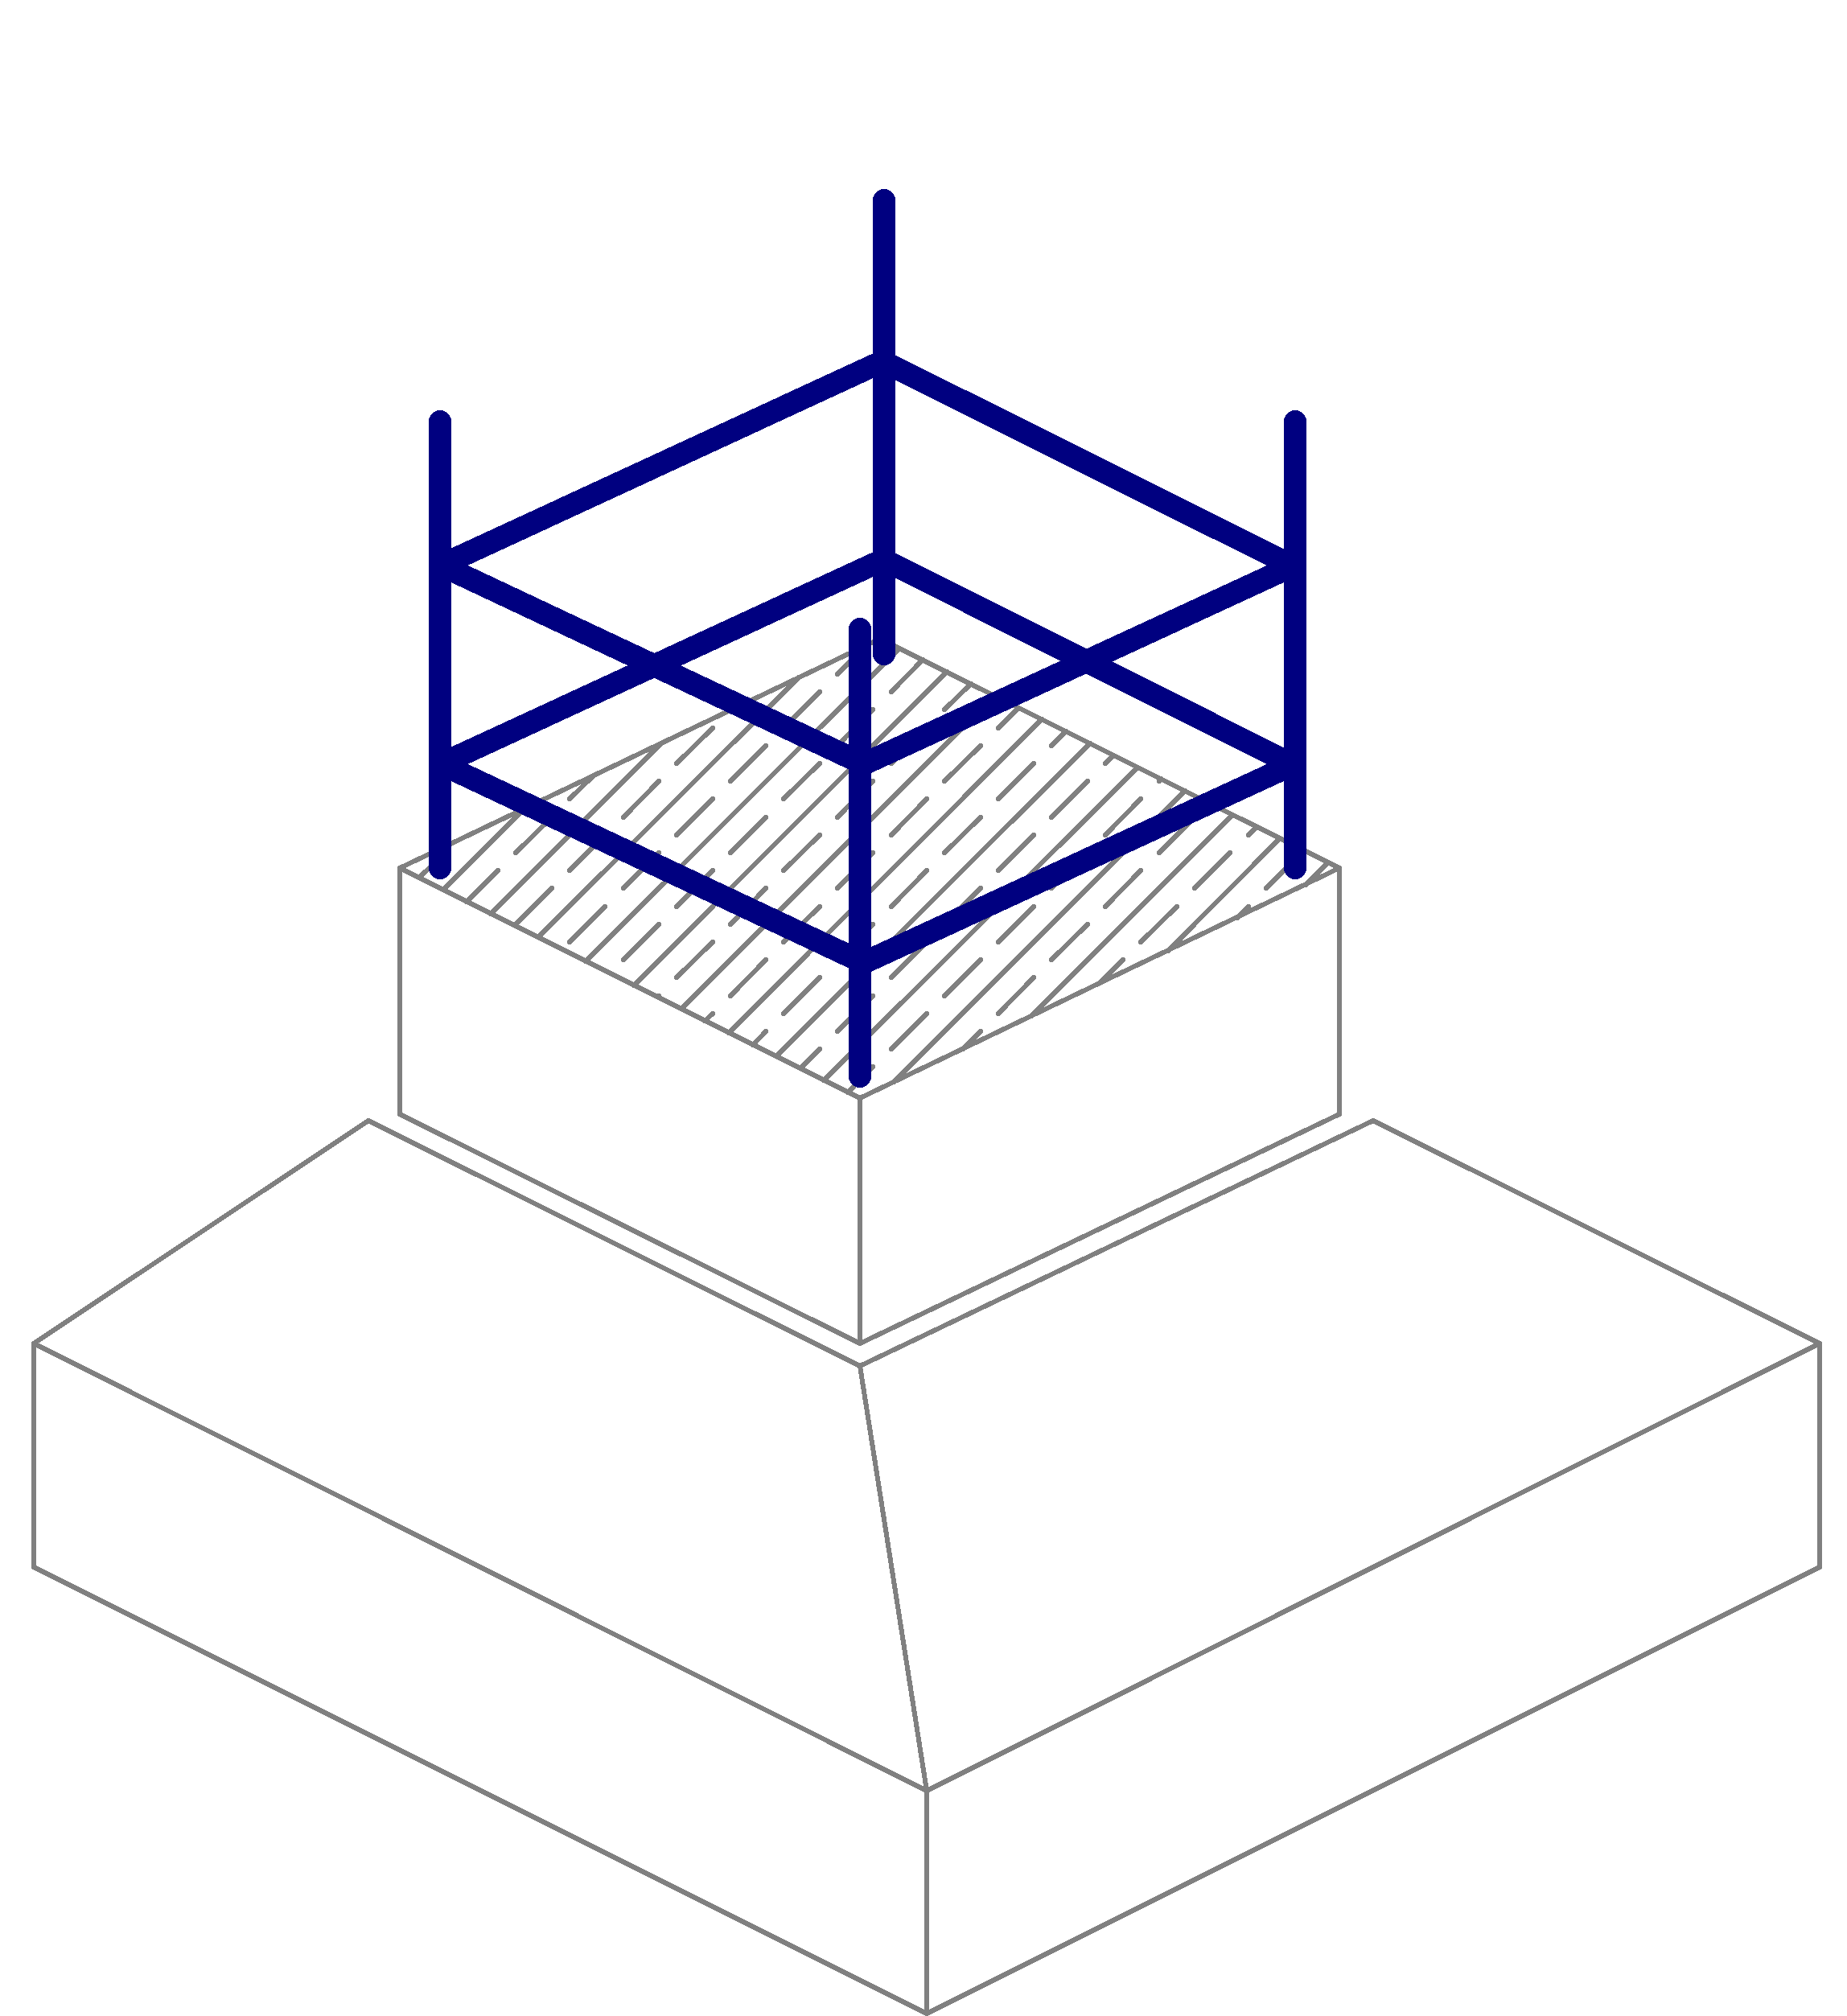
\includegraphics[width=0.4\textwidth]{Fundacoes-rasas-ou-diretas/Imagens/Sapata-isolada-1.png}
	\end{center}
\end{figure}

Para o pré-dimensionamento de altura de uma sapata, pode-se utilizar a seguinte equação:

\begin{equation}
	h=30\%\cdot a
\end{equation}

Alguns \textbf{critérios de projeto} devem ser considerados no pré-dimensionamento de sapatas isoladas:

\begin{enumerate}
	\item O centro de gravidade da sapata deverá coincidir com o centro de carga dos pilares; $${CG}_{sapata}={CG}_{pilar}$$
	\item Nenhuma dimensão da sapata deverá ser inferior a 60 $cm$; $$b\geqslant60\;cm$$
	\item A relação entre os lados da sapata não deverá ultrapassar a 2,5; $$\frac{a}{b}\leqslant2,5$$
	\item Os balanços da sapata deverão ser iguais nas duas direções ortogonais da peça.\begin{equation}\label{equacao-equilibrio-balancos}a-a_0=b-b_0\end{equation}
\end{enumerate}

Observações:

\begin{enumerate}
	\item Quando o somatório das áreas das sapatas ultrapassar 50\% da área da projeção da edificação no terreno, deve-se trocar a solução \textbf{sapata isolada} por \textbf{radier};
	\item Ao escolher o tipo de fundação a ser adotado em um projeto, deve-se testar, \textbf{primeiramente}, a solução \textbf{sapata isolada}. Caso não seja possível, deve-se partir para outras alternativas, inclusive \textbf{fundações profundas}.
\end{enumerate}

A figura a seguir ilustra o caso de \textbf{sapatas em terrenos inclinados}. Percebe-se que uma nova sapata deve ficar no mínimo a uma distância $b$ da sapata já construída.

*Inserir imagem

Exemplo: Dimensionar as sapatas para os pilares P1 e P2 com as seguintes características:
P1 (30x30) $cm\rightarrow$ 3000 $kN$; P2 (30x60) $cm\rightarrow$ 4200 $kN$; $\sigma_s=0,3\;MPa$.

Para \textbf{P1}:

Como $a_0=b_0$, a sapata será quadrada ($a=b$). $$A=b\cdot b$$ $$A=b^2$$

Como $A=\frac{P}{\sigma_s}$, tem-se:

$$b=\sqrt{\frac{P}{\sigma_s}}=\sqrt{\frac{3000\;kN}{300\;\frac{kN}{m^2}}}\approx3,162\;m\approx3,2\;m$$

Portanto, a altura $h$ da sapata é $h=30\%\cdot a=30\%\cdot 3,2=0,96\approx0,95$

Nota-se que foi arredondado para baixo. Pode-se fazer isso quando os arredondamentos de $a$ e $b$ forem mais folgados e consequentemente não atrapalharem na quantidade de área. Se fosse utilizado $h=0,95\;m$, fazendo a conta inversa, obteria-se um $a=0,95/0,3\approx3,17\;m\approx3,2\;m$.

Para \textbf{P2}:

O pilar é retangular, indicando que as dimensões da sapata também serão.
$$A=\frac{P}{\sigma_s}=\frac{4200\;kN}{300\;\frac{kN}{m^2}}=14\;m^2$$

Como $A=a\cdot b$:
$$a=14\;m^2/b$$

Para que os momentos fletores sejam iguais nas duas direções ortogonais, tem-se:
$$a-a_0=b-b_0$$
$$\frac{14}{b}-0,6=b-0,3$$

Multiplicando todos os elementos por $b$:
$$14-0,6b=b^2-0,3b$$

Igualando toda a equação a zero, tem-se:
$$b^2+0,3b-14=0$$

Encontrando-se as raízes por Bhaskara:
$$x_{1, 2}=\frac{-b\pm\sqrt{b^2-4\cdot a\cdot c}}{2\cdot a}=\frac{-0,3\pm\sqrt{0,3^2-4\cdot 1\cdot (-14)}}{2\cdot1}$$
$$x_1\approx3,59\;m$$
$$x_2\approx-3,89\;m$$

Voltando, tem-se:
$$a=\frac{14\;m^2}{b}=\frac{14\;m^2}{3,59\;m}\approx3,89\;m\approx3,9\;m$$

Percebe-se que as duas raízes da equação correspondem aos lados da sapata, sendo uma delas em módulo. A altura $h$ é, portanto:
$$h=30\%\cdot a=30\%\cdot 3,9\;m=1,17\;m\approx1,2\;m$$

As dimensões das sapatas isoladas são: P1 ($a=b=3,2\;m$ e $h=0,95\;m$); e P2 ($a=3,9\;m$, $b=3,6\;m$ e $h=1,2\;m$).